%%% Document Formatting
\documentclass[12pt,fleqn]{article}
\usepackage[a4paper,
            bindingoffset=0.2in,
            left=0.75in,
            right=0.75in,
            top=0.8in,
            bottom=0.8in,
            footskip=.25in]{geometry}
\setlength\parindent{10pt} % No indent

%%% Imports
% Mathematics
\usepackage{amsmath} % Math formatting
\numberwithin{equation}{section} % Number equation per section
\DeclareMathOperator{\Tr}{Tr}


\newtheorem{theorem}{Theorem}
\newtheorem{definition}{Definition}
\newtheorem{proof}{Proof}
\newtheorem{lemma}{Lemma}
\newtheorem{example}{Example}

\usepackage{amsmath}
\usepackage{amsfonts} % Math fonts
\usepackage{amssymb} % Math symbols
\usepackage{mathtools} % Math etc.
\usepackage{slashed} % Dirac slash notation
\usepackage{cancel} % Cancels to zero
\usepackage{empheq}
\usepackage{breqn}

\newcommand{\expect}[1]{\mathbb{E}\left[#1\right]}


% Visualization
\usepackage{graphicx} % for including images
\graphicspath{ {} } % Path to graphics folder
\usepackage{tikz}



%%% Formating
\usepackage{hyperref} % Hyperlinks
\hypersetup{
    colorlinks=true,
    linkcolor=blue,
    filecolor=magenta,      
    urlcolor=cyan,
    pdftitle={Overleaf Example},
    pdfpagemode=FullScreen,
    }
\urlstyle{same}

\usepackage{mdframed} % Framed Enviroments
\newmdenv[ 
  topline=false,
  bottomline=false,
  skipabove=\topsep,
  skipbelow=\topsep
]{sidework} %% Side-work

\usepackage{lipsum} % Lorem Ipsum example text

%%%%% ------------------ %%%%%
%%% Title
\title{Speciation Time \& Classifier Free Guidance}
\author{Clark Miyamoto (cm6627@nyu.edu)}
\date{\today}
\begin{document}

\maketitle

\tableofcontents

\section{Introduction}
I recently learned about Speciation Time $t_S$ from a lecture given by Marc Mezard at the Beg Rohu Summer School. To me this gives a better mathematical basis for some work done by Matthieu Wyart \href{https://www.pnas.org/doi/full/10.1073/pnas.2408799121}{"A phase transition in diffusion models reveals the hierarchical nature of data"}. Basically he shows if you add increasing strength of noise to an image, then run it through a diffusion model, it'll affect small features of the image, and then eventually change the whole class.\\

So for example, you start with a image of a cat, add some noise then de-noise, it becomes a leopard, do that again it becomes a bear, then a moth. 
\\

Wyart does this empirically (although he does give a theoretical model which connects replicates this transition, it seems a little cooked up to me, like where is the score?). I think it'd be interesting to see if we can derive this phenomena completely 

\section{Speciation Time}

There are three dynamical regimes in the time-reversed process (in the liit of large number of data \& large dimension)
\begin{enumerate}
	\item \emph{Regime I:} At the beginning of the backward process, the random dynamical trajectories have not committed to a particular class of data.
	\item \emph{Regime II:} Trajectories have committed to a particular class, and will stay until the ned of the backwards process.
	\item \emph{Regime III:} There is no generalization, but instead diffusion models display memorization of the training set.
\end{enumerate}

\subsection{Derivation of Speciation Time}
Let $\mathcal D = \{\vec a^\mu\}_\mu$ denote the set of training samples, which we assume were sampled iid from $p_0(\vec a)$. We can noise our samples using an OU (variance-preserving) process,
\begin{align}
	x_t = \sqrt{e^{-2t}} a + \sqrt{1-e^{-2t}} \eta, ~~ \eta \sim \mathcal N(0, \mathbb I)
\end{align}
In my notation, the forward process $t \to \infty$ is white noise (base distribution), and the reverse process $t \to 0$ is the data (target distribution). Also for future reference, I'll notate the noise variance as $\Delta_t = 1- e^{-2t}$.\\
\\
Let's talk about the probability distributions $p(x_t | a)$.  Since this is just two random variables being added, the probability distribution gets convolved:
\begin{align}
	p_t(\vec x) & = \int d\vec a ~p(\vec x | \vec a) p(\vec a)  \\
	& = \int d \vec a ~ p_0(\vec a)  \frac{1}{\sqrt{2\pi \Delta_t}^d} \exp \left (- \frac{1}{2} \frac{(\vec x - \vec a e^{-t})^2}{\Delta_t} \right)
\end{align}
where 
\begin{align}
	p_t(\vec x)  & = \frac{1}{\sqrt{2\pi \Delta_t}^d} \exp \left ( - \frac{1}{2} \frac{\vec x^2}{\Delta_t} + g(\vec x) \right)
\end{align}
where
\begin{align}
	g(\vec x) = \log \int d\vec a~ p_0(\vec a) \exp \left (- \frac{1}{2} \frac{\vec a^2 e^{-2t}}{\Delta_t} \right) \exp \left( \frac{e^{-t}}{\Delta_t} \vec x \cdot \vec a\right)
\end{align}
\begin{sidework}
	\emph{We will now work in the large-time limit $t \gg 1$ (near base distribution)}.\\
	\\
	Let $\langle \cdot \rangle$ denote expectation value w.r.t. the effective distribution $p_0(\vec a) \exp(-\frac{\vec a^2 e^{-2t}}{2\Delta_t})$, which in the large time limit is effectively $p_0(\vec a)$. \\
	\\
	We'll start by Taylor expanding the 2nd exponential $\exp(\frac{e^{-t}}{\Delta_t} \vec x \cdot \vec a) \approx 1 + \frac{e^{-t}}{\Delta_t} \vec x\cdot \vec a + ...$
\begin{align}
	g(\vec x) = \log \left (1 + \frac{e^{-t}}{\Delta_t} \vec x \cdot \langle \vec a \rangle  + \frac{1}{2} \frac{e^{-2t}}{\Delta_t^2} \langle (\vec x  \cdot \vec a)^2 \rangle +  \mathcal O(x e^{-t})^3\right)
\end{align}
And now Taylor expand the $\log (1+x) \approx x - x^2/2 + \mathcal O(x^3)$
\begin{align}
	g(\vec x) & = \frac{e^{-t}}{\Delta_t} \vec x \cdot \langle \vec a \rangle  + \frac{1}{2} \frac{e^{-2t}}{\Delta_t^2} \langle (\vec x  \cdot \vec a)^2 \rangle - \frac{1}{2} \left( \frac{e^{-t}}{\Delta_t} \vec x \cdot \langle \vec a \rangle  + \frac{1}{2} \frac{e^{-2t}}{\Delta_t^2} \langle (\vec x  \cdot \vec a)^2 \rangle\right)^2 + \mathcal O(x e^{-t})^3\\
	& = \frac{e^{-t}}{\Delta_t} \vec x \cdot \langle \vec a \rangle  + \frac{1}{2} \frac{e^{-2t}}{\Delta_t^2} \left[\langle (\vec x \cdot \vec a )^2\rangle - (\vec x \cdot \langle \vec a \rangle)^2 \right] + \mathcal O(x e^{-t})^3\\
	& = \frac{e^{-t}}{\Delta_t} \sum_{i=1}^d x_i \langle a_i\rangle + \frac{1}{2} \frac{e^{-2t}}{\Delta_t}  \sum_{ij=1}^d x_i x_j [ \langle a_i a_j\rangle - \langle a_i \rangle \langle a_j\rangle] + \mathcal O(x e^{-t})^3
\end{align}
\end{sidework}
Plugging this approximation into $p_t(\vec x)$
\begin{align}
	\log p_t(\vec x) & = C + \frac{e^{-t}}{\Delta_t} \sum_i x_i \langle a_i\rangle - \frac{1}{2\Delta_t} \sum_{ij} x_i M_{ij} x_j + \mathcal O(x e^{-t})^3\\
	\text{s.t. } M_{ij} & = \delta_{ij}  - e^{-2t} [\langle a_i a_j\rangle - \langle a_i \rangle \langle a_j\rangle]
\end{align}
Interpreting the matrix $M$, a couple things to note
\begin{enumerate}
	\item That second term, that's just the empirical covariance matrix of the data! That is $\langle a_i a_j\rangle - \langle a_i \rangle \langle a_j\rangle = \Sigma_{ij}$
	\item This is actually just the Hessian of $\log p_t(\vec x)$ (in the limiting case $t \gg 1$, near target distribution). 
	\item If the Hessian of $\log p_t(\vec x)$ is positive-semi-definite, then the distribution is log concave. Imagine the target distribution is multimodal (i.e. multiple classes, dog image vs cat image), so while it's still log-concave, we can think of this as the samples not committing to a particular mode.
\end{enumerate}
When $\log p_t(x)$ is no longer convex, meaning samples have committed to a path, I'd like to give that a special name. We'll denote this time as $t_S$ the \textbf{speciation time}. \\
\\
We can derive this by figuring out when the Hessian $M$ is no longer positive-semi-definite. You can do this via operator norm, this gets ya $e^{-2t_s} \leq || \Sigma||_2^{-1}$. Writing it out in a nice way:
\begin{align}
	\boxed{t_s = \frac{1}{2} \log \lambda_{max}(\Sigma)}
\end{align}

\section{Classifier Free Guidance}
Consider generating samples using Langevin dynamics
\begin{align}
	dx_\tau = x_\tau d\tau + 2 s_\tau (x) + \sqrt{2} dB_\tau \label{eqn:Lagevin}
\end{align}
where $\tau = t_f - t$ denotes the reverse time, and $s_\tau(x) =\nabla_x \log p_t(x)$ is the score.\\
\\
Classifier Free Guidance does not do that, rather it directs the diffusion in a manner proportional to the difference between the conditional and unconditional score.
\begin{align}
	s^{CFG}_t(x | c) & = s_t(x | c)+ \omega [s_t(x | c) - s_t(x)]\\
	& \nabla_x \big(\log p_t(x|c) - \omega [\log p_t(x|c) - \log  p_t(x)]\big)
\end{align}
So to generate samples, you get your lagenvin dynamics equation (\ref{eqn:Lagevin}) and swap out $s_\tau(x)$ for $s^{CFG}_t(x | c)$.\\
\\
CFG offers practical advantages (i.e. works on unlabeled data), however  a key question remains: "Is CFG is capable of accurate generating samples from the target distribution?"

\subsection{Worked Example: Symmetric Gaussian Mixtures}
\subsubsection{Setup}
Consider a mixture of two $d$-dimensional gaussians centered at $\pm \vec \mu$
\begin{align}
	p_0(\vec x) = \frac{1}{2(\sqrt{2 \pi \sigma^2})^d} \left ( e^{-(\vec x - \vec \mu)^2 / 2 \sigma^2} + e^{-(\vec x + \vec \mu)^2  / 2\sigma^2} \right)
\end{align}
Noising this with an OU process, we find the probability $p_t(\vec x)$
\begin{align}
	p_t(\vec x) & = \frac{1}{2(\sqrt{2\pi \Gamma_t})^d}  \left ( e^{-(\vec x - \vec \mu e^{-t})^2 / 2 \Gamma_t^2} + e^{-(\vec x + \vec \mu e^{-t})^2  / 2\Gamma_t^2} \right)\\
	\log p_t(\vec x) & = - \frac{\vec x^2}{2 \Gamma_t} + \log \cosh \left (\vec x \cdot \vec \mu \frac{e^{-t}}{\Gamma_t} \right) + \text{Constant w.r.t. } \vec x\\
	\nabla_x \log p_t(\vec x)& = - \frac{\vec x}{\Gamma_t} + \vec \mu \frac{e^{-t}}{\Gamma_t} \tanh\left(\vec x \cdot \vec \mu \frac{e^{-t}}{\Gamma_t} \right)
\end{align}
where $\Gamma_t = \sigma^2 e^{-2t} + \Delta_t$
We can also ask, what's the conditional distribution's score
\begin{align}
	\nabla_x \log p_t(\vec x | \pm\vec \mu)  = \frac{-\vec x \pm \vec \mu e^{-t}}{\Gamma_t}
\end{align}
Plugging this into the CFG score, we get
\begin{align}
	s_t^{CFG}(x|c=  \pm \mu )& = \frac{-x \pm \mu e^{-t}}{\Gamma_t} + \omega [\frac{-x \pm \mu e^{-t}}{\Gamma_t}+ \frac{x}{\Gamma_t} + \mu \frac{e^{-t}}{\Gamma_t} \tanh(x^T \mu \frac{e^{-t}}{\Gamma_t} )]
\end{align}
Rearranging, we can see that the residual that CFG has from the true conditional score
\begin{align}
	s_t^{CFG}(x |c = \pm \mu) - s_t(x|c = \pm \mu) & = \underbrace{\mu ~ \omega \frac{e^{-t}}{\Gamma_t}  [\pm 1 +  \tanh(x^T \mu \frac{e^{-t}}{\Gamma_t} )]}_{\text{score gap}}
\end{align}
\subsubsection{Speciation Time}
We can now ask our self, what is the role of CFG at different times? The only natural time-scale we have is the speciation time, so we can ask, what happens before, at, and after?\\
\\
To get there, we need to compute the speciation time.
\begin{align}
	t_S = \frac{1}{2} \log \lambda_{max}(\Sigma)
\end{align}
The covariance has a simple expression
\begin{align}
	\Sigma & = \mathbb E[XX^T] - \underbrace{\mathbb E[X] \mathbb E[X^T]}_{0, \text{ by symmetry}}\\
	& = \Sigma + \mu \mu^T\\
	& = \sigma^2 \mathbb I + \mu \mu^T & \text{We choose unit covariance WLOG}
\end{align}
The highest eigenvalue is $\lambda_{max}(\sigma) = \sigma^2 + \| \mu\|^2 := \sigma^2 + d ~ \tilde \mu^2$. You should interpret $\tilde \mu$ as the per-coordinate RMS $\tilde \mu \equiv \| m \| / \sqrt{d}$. They choose this because you assume the entires of $\mu$ are iid with variance order 1. 
\begin{sidework}
	You can interpret this as you're getting more information as your data distribution gains more dimension (i.e. images w/ more resolution). You can choose the scaling $\tilde \mu \sim \mathcal O(1/\sqrt{d})$ if you want to make statements that you don't learn more information as you gain more dimensions...\\
	\\
	Their asymptotic results will vary depending on this parameterization...
\end{sidework}
Therefore the speciation time for this problem is 
\begin{align}
	t_S = \frac{1}{2} \log d + \frac{1}{2} \log \left(\mu^2 + \frac{\sigma^2}{d} \right)
\end{align}
In the paper, they analyze this in the $d \gg 1$ limit, yielding $t_S = \frac{1}{2 } \log d$.
\subsubsection{Discussion}
Generically, we'll do all this analysis in the direction $q := x \cdot \hat \mu$. This is because the trasverse direction (directions orthogonal to $\mu$) don't have interesting dynamics.\\
\\
\textbf{Before Speciation Time $t_S$}

\begin{sidework}
	Let's analyze what CFG does prior to speciation time (meaning $t \gg 1$). In this limit $\Gamma_t = 1 - e^{-2t} \approx 1$.  The only interesting dynamics occurs in the $\hat m = \vec \mu / \|\mu\|$ direction.
	\begin{align}
		\vec s_t^{CFG} \cdot \hat m
	\end{align}
	Now let's plot the negative log probability in this direction $\vec x \cdot \hat m := q$
	\begin{align}
		- \log p_\tau^{CFG}(q | c = \pm \mu) = \underbrace{(\frac{1}{2}q^2 \mp q \|\mu\| e^{-\tau})}_{\text{Classifier's Log Prob}} + \omega \|\mu\| \underbrace{\left[ \mp q e^{-\tau} + \log \cosh (q \|\mu\|e^{-\tau})\right]}_{\text{Extral Log Prob due to CFG}} + \text{Constant}
	\end{align}
	See an interactive plot of this at \url{https://www.desmos.com/calculator/vao4sxx6ss}.\\
	\\
	Notice, when $\omega \neq 0$, you don't recover the correct mean. 
\end{sidework}
Takeaway: \textbf{Prior to speciation time, CFG aids in speeding up convergences to the target class.}\\
\\
\textbf{Right before speciation time:}\\
The takeaway: \textbf{Right before speciation time, the guided path $s^{CFG}(x|c)$ realigns with the unguided path $s(x|c)$ which generates the correct conditional distribution.}
\\
\\
\textbf{After Speciation Time}\\
After speciation time, samples have committed to a class / path. Hence they are aligned with the mode $x \cdot m \sim \mathcal O(d)$, therefore $c - \tanh\left(x \cdot m  \tfrac{e^{-t}}{\Gamma_t} \right) \approx 0$. Therefore the score gap $\delta s_t \approx 0$, meaning the CFG score well approximates the correct conditional score $s^{CFG}(x|c) \approx s(x|c)$.\\
\\
The take away: \textbf{after speciation time, extra corrections from the guidance turn off}.

\subsection{Generic Claims}
\begin{enumerate}
	\item \textbf{When is guidance helpful:} In the two gaussian mixture, the score gap $\delta s_t(x) = \| \nabla_x \log p_t(x | c) - \nabla_x \log p_t(x)\|$ is tiny at the start (both look like gaussian noise), then increases during regime I (prior to speciation, class undecided), and then collapses back to zero after speciation (class decided).  So, \textbf{guidance should be on in regime I, and then switch off near/after the speciation time $t_S$}. 
	\item Bias of traditional CFG: The residual of the CFG score and true conditional score is linear w.r.t. $\delta s_t$
	\begin{align}
		s^{CFG}_t(x) & = s_t(x|c) + \omega [s_t(x|c) - s_t(x)]\\
		s^{CFG}_t(x) - s_t(x|c) & = \omega [s_t(x|c) - s_t(x)]\\
		\| s^{CFG}_t(x) - s_t(x|c) \| & = |\omega| \delta s_t
	\end{align}
	In our treatment of the gaussian mixture (in finite dimension), we saw $\delta	s_t \sim \mathcal O(d^{-1/2})$ (didn't vanish quick enough). So we want a scheme which (exponentially) suppresses $\delta s_t$. The take away is to \textbf{not keep a linear push when $\delta s_t$ is small}.
	\item Combining (1, guidance help in regime I \& switch off) and (2, dampen when guidance shouldn't act) 
	\begin{align}
		S^{NL-CFG}_t(x) - s_t(x|c)  = [s_t(x|c) - s_t(x)] \phi_t(\delta s_t)
	\end{align}
	where $\lim_{x \to 0} x \phi_t(x) = 0$ (ensures (2)). To ensure (1) we just have to cook up the correct $\phi_t$ which has an amplifying affect.
\end{enumerate}
The authors propose using a power-law guidance $\phi_t(x) = \omega x^\alpha$ (where $\alpha > -1$, to satisfy the limit condition).

\newpage
\section{Results}
\subsection{Numerics of Gaussian Mixture Model}
\begin{figure*}[h]
	\centering
	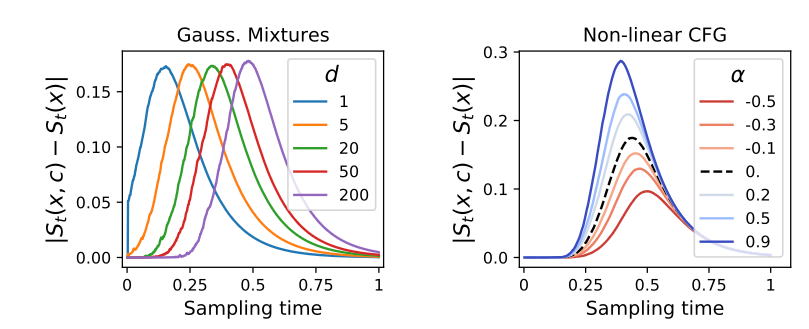
\includegraphics[scale=0.5]{powerlaw.png}
	\caption{This is Figure 4 in Kruno's paper. They do the symmetric gaussian mixture model that I talked about, and do $s_{t}^{CFG}(x(t) | c)$ where the trajectory $x(t)$ is generated by Langevin Dynamics $dx_t = (x_t + 2 s_t^{CFG}(x_t|c)) dt + \sqrt{2} dW_t$. They plot the projection $x \cdot \hat m$.}
\end{figure*} 

\subsection{Images (cause of a diffusion paper isn't complete without images)}
See all images on the paper (duh), but here's a screenshot of nice examples.
\begin{figure*}[h]
	\centering
	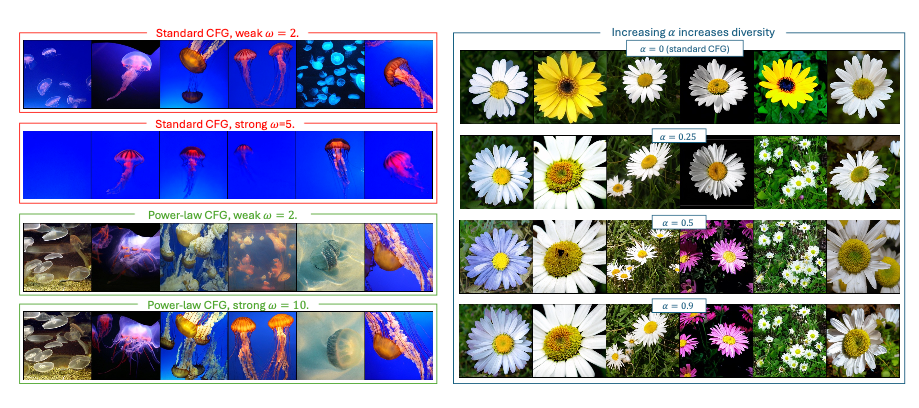
\includegraphics[scale=0.5]{realdata.png}=
\end{figure*}











\end{document}